\chapter{Design}

\section{Use case: Skriv besked}

Fokus har i dette sprint v�ret p� funktionaliteten, som tillader brugeren at skrive en besked i g�stebogen. Beskeden skal efterf�lgende kunne vises i brugergr�nsefladen og gemmes til en fil, som kan indl�ses, n�r programmet �bnes n�ste gang.

\begin{figure}[H]
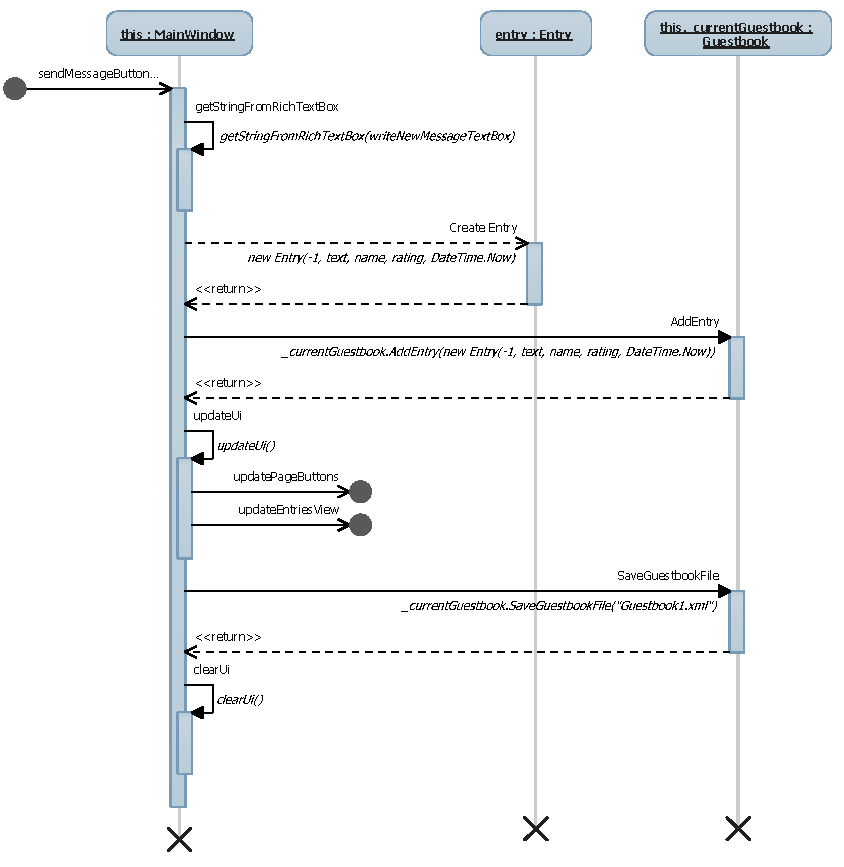
\includegraphics[width=\linewidth]{./add-entry-ssd}
\caption{Systemsekvensdiagram for AddEntry}
\label{add-entry-ssd}
\end{figure}

Figur \ref{add-entry-ssd} viser systemsekvensdiagrammet for AddEntry-metoden.

De 3 centrale skridt i operationen, som er knyttet til dom�nelogikken, er:

\begin{itemize}
\item Opret Entry-objektet
\item Tilf�j Entry-objektet til g�stebogen
\item Gem g�stebogsfilen
\end{itemize}

Det f�rste skridt er et simpelt \emph{constructor}-kald, og vi vil derfor ikke g� i dybden med det. 

Det n�ste skridt er at tilf�je beskeden til g�stebogen. 
 
\begin{figure}[H]
\caption{Operationskontrakt for AddEntry}
\label{add-entry-contract}
\begin{itemize}
\item[]
\item[] \textbf{Use-case:} Skriv en besked til g�stebogen
\item[] \textbf{Operation:} AddEntry(navn, besked: String, vurdering: Int, dato: Date)
\item[] \textbf{Pre:} Navn, vurdering og besked er udfyldt
\item[] \textbf{Post:} Et unikt ID er genereret og beskeden er tilf�jet til g�stebogen
\item[] \textbf{Output:} Brugeren g�res opm�rksom p� at beskeden er tilf�jet
\end{itemize}
\end{figure}

Figur \ref{add-entry-contract} viser operationskontrakten for denne metode.

\begin{figure}[H]
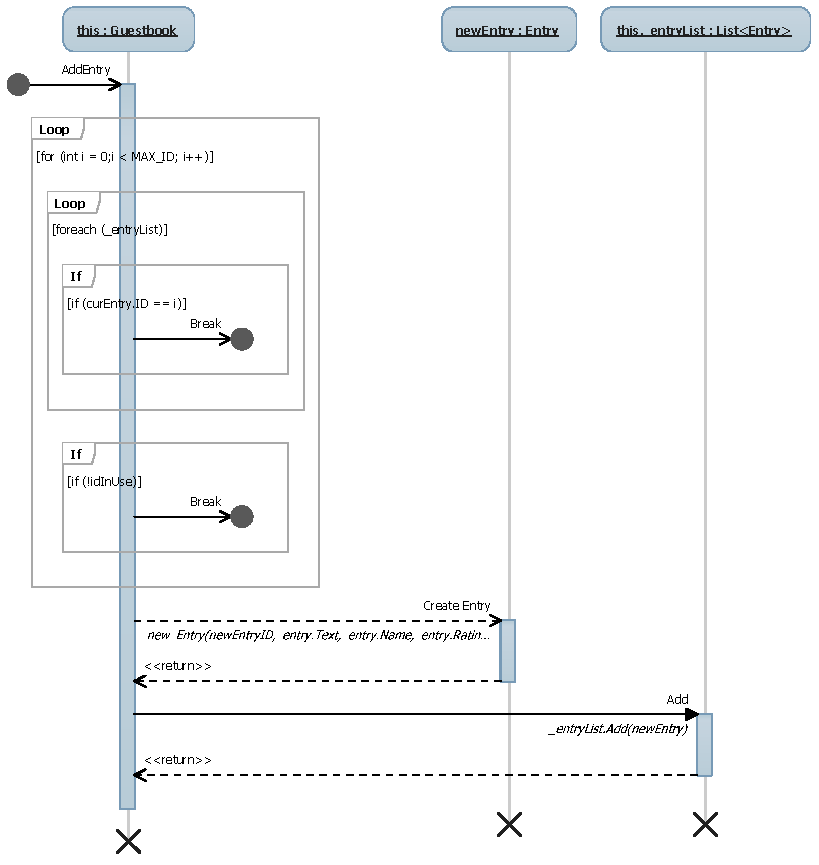
\includegraphics[width=\linewidth]{./add-entry-sd}
\caption{Sekvensdiagram for AddEntry}
\label{add-entry-sd}
\end{figure}

Den centrale funktionalitet i denne metode er at generere et unikt ID til beskeden. Figur \ref{add-entry-sd} viser sekvensdiagrammet for denne metode.

\begin{figure}[H]
\caption{Operationskontrakt for SaveGuestbookFile}
\label{save-guestbook-file-contract}
\begin{itemize}
\item[]
\item[] \textbf{Use-case:} Skriv en besked til g�stebogen
\item[] \textbf{Operation:} SaveGuestbookFile(filnavn : String)
\item[] \textbf{Pre:} Et filnavn er valgt for den nuv�rende g�stebog
\item[] \textbf{Post:} G�stebogen er gemt i Xml-format til harddisken
\item[] \textbf{Output:} Intet
\end{itemize}
\end{figure}

Det sidste skridt er at gemme g�stebogsfilen til harddisken. Figur \ref{save-guestbook-file-contract} viser operationskontrakten for denne metode.

\begin{figure}[H]
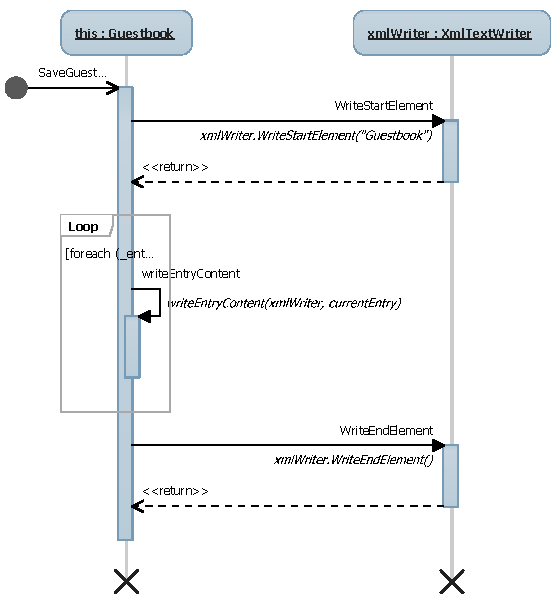
\includegraphics[width=\linewidth]{./save-guestbook-file-sd}
\caption{Sekvensdiagram for SaveGuestbookFile}
\label{save-guestbook-file-sd}
\end{figure}

Figur \ref{save-guestbook-file-sd} viser sekvensdiagrammet for denne metode.

\section{Use case: Skjul besked}

Funktionaliteten for administration er endnu ikke implementeret i systemet, men vi har udarbejdet operationskontrakter for de centrale metoder. Figur \ref{hide-entry-contract} viser operationskontrakten for funktionaliteten som tillader at skjule en besked i g�stebogen.

\begin{figure}[H]
\caption{Operationskontrakt for HideEntry}
\label{hide-entry-contract}
\begin{itemize}
\item[]
\item[] \textbf{Use-case:} Administratoren skjuler en besked i g�stebogen
\item[] \textbf{Operation:}  HideEntry(navn, besked: String, vurdering: Int, dato: Date)
\item[] \textbf{Pre:} Beskeden er valgt 
\item[] \textbf{Post:} Beskeden er skjult
\item[] \textbf{Output:} Beskeden er nu blivet skjult
\end{itemize}
\end{figure}

\section{Use case: Slet besked}

Figur \ref{delete-entry-contract} viser operationskontrakten for funktionaliteten som tillader at slette en besked fra g�stebogen.

\begin{figure}[H]
\caption{Operationskontrakt for DeleteEntry}
\label{delete-entry-contract}
\begin{itemize}
\item[]
\item[] \textbf{Use-case:} Administrator sletter en besked fra g�stebogen
\item[] \textbf{Operation:} DeleteEntry(navn, besked: String, id, vurdering: Int, dato: Date)
\item[] \textbf{Pre:} Der er valgt en besked
\item[] \textbf{Post:} Den valgte besked bliver slettet fra g�stebogen
\item[] \textbf{Output:} "Beskeden er slettet"
\end{itemize}
\end{figure}

\section{Use case: Skift g�stebog}

Figur \ref{change-guestbook-contract} viser operationskontrakten for funktionaliteten som tillader at �ndre, hvilken g�stebog, som skal v�re aktiv.

\begin{figure}[H]
\caption{Operationskontrakt for ChangeGuestbook}
\label{change-guestbook-contract}
\begin{itemize}
\item[]
\item[] \textbf{Use-case:} Administratoren v�lger hvilken g�stebog der er aktuelt vist for brugeren
\item[] \textbf{Operation:} ChangeGuestbook(G�stebog: Guestbook)
\item[] \textbf{Pre:} Den aktuelle g�stebog er valgt
\item[] \textbf{Post:} G�stenbogen er blevet valgt
\item[] \textbf{Output:} Du har nu valgt en ny g�stebog
\end{itemize}
\end{figure}